% Created 2018-05-20 Sun 17:40
% Intended LaTeX compiler: pdflatex
\documentclass[11pt]{article}
\usepackage[utf8]{inputenc}
\usepackage[T1]{fontenc}
\usepackage{graphicx}
\usepackage{grffile}
\usepackage{longtable}
\usepackage{wrapfig}
\usepackage{rotating}
\usepackage[normalem]{ulem}
\usepackage{amsmath}
\usepackage{textcomp}
\usepackage{amssymb}
\usepackage{capt-of}
\usepackage{hyperref}
\renewcommand{\thesection}{\Roman{section}}
\renewcommand{\thesubsection}{\thesection.\Roman{subsection}}
\renewcommand{\thesubsubsection}{\thesubsection.\Roman{subsubsection}}
\usepackage[parfill]{parskip}
\usepackage{color}
\usepackage{amsmath}
\usepackage{amssymb}
\usepackage{pgfplots}
\usepackage{mathtools}
\date{\today}
\title{}
\hypersetup{
 pdfauthor={},
 pdftitle={},
 pdfkeywords={},
 pdfsubject={},
 pdfcreator={Emacs 27.0.50 (Org mode 9.1.9)}, 
 pdflang={English}}
\begin{document}

\tableofcontents

\newpage

\section{Die kurze Frist}
\label{sec:orgeeee47f}
\begin{itemize}
\item kombinierter Einsatz von Geld- und Fiskalpolitik\\
\end{itemize}

Zentrale Frage: \textbf{Wie hoch ist die Güterproduktion?}\\
-> Antworten aus der Keynesianischen Theorie:
\begin{itemize}
\item die Güterproduktion (Angebot) wird allein durch die Nachfrage bestimmt
\item angebotsseitige Einflüsse wie bswp Technologie und Qualifikation der Arbeitskräfte können vernachlässigt werden, weil die Nachfrage das Angebot nicht ausschöpft
\item Annahme dass Güterpreise konstant sind
\end{itemize}

Güternachfrage hängt von vielen Faktoren ab, u.a. vom \textbf{Gütermarkt} und dem Geschehen auf \textbf{Geld- und Finanzmärkten}. Im Folgenden daher Betrachtung von:
\begin{enumerate}
\item Gütermarkt
\begin{itemize}
\item Untersuchung des Gleichgewichts auf dem Gütermarkt
\item Beschreibung der \textbf{nachfrageseitigen} Bestimmung von Produktion und Einkommen
\item Analyse des Einflusses der Fiskalpolitik
\end{itemize}

\item Geld- und Finanzmärkte
\begin{itemize}
\item Untersuchung des Gleichgewichts auf den Geld- und Finanzmärkten
\item Beschreibung der Bestimmung des Zinses
\item Analyse des Einflusses der Geldpolitik
\end{itemize}

\item IS-LM-Modell
\begin{itemize}
\item Untersuchung des Zusammenwirkens von Güter-, Geld- und Finanzmärkten
\item Beschreibung der simultanen Bestimmung von Produktion \& Einkommen, sowie des Zinses
\begin{itemize}
\item dies bezeichnet man als IS-LM-Modell
\end{itemize}
\end{itemize}
\end{enumerate}

\subsection{Der Gütermarkt}
\label{sec:org751765f}
Markteilnehmer auf em Gütermarkt sind die volkswirtschaftl. Sektoren (Haushalte, Staat, Unternehmen)

\textbf{Makroökonomischer Gütermarkt=} (gedachte) Zusammenfassung aller Güterkäufe und -verkäufe in einem Land innerhalb 1 Periode (\(\approx\) BIP)

Angebot = inländische Produktion + Ausland(Import) = Y + IM

Nachfrage = Haushalte + Unternehmen + Staat + Ausland(Export) = C + I + G + X

Die Konsumausgaben (Nachfrage) der privaten Haushalte (C -> Consumers) entspricht allen Waren \& Dienstleistungen, die von Verbrauchern gekauft werden

Die Konsumausgaben (Nachfrage) des Staates (G -> Government) entspricht allen Waren \& Dienstleistungen, die durch den staatlichen Sektor (Bund, Länder und Gemeinden) gekauft werden.

Die Investitionen also die "Nachfrage" der Unternehmen (I) setzen sich zusammen aus Anlageinvestitionen (= gewerbliche Investitionen, Wohnungsbauinvestitionen) und Lagerinvestitionen (= Vorratsänderungen). Die Vorratsänderungen werden in unserem Modell zunächst vernachlässigt (Wert also gleich Null).
Die Investitionen lassen sich "brutto" (einschließlich Abschreibungen) und "netto" (ohne Abschreibungen) erfassen. Ergo entsprechen Bruttoinvestitionen = Nettoinvestitionen plus Abschreibungen. Abschreibungen vernachlässigen wir in diesem Modell jedoch auch zunächst (Wert gleich Null).

Die Exporte (X) entsprechen dem Kauf einheimischer Waren \& Dienstleistungen durch Ausländer.
Die Importe (IM) entsprechen dem Kauf ausländischer Waren \& Dienstleistungen durch einheimische Konsumenten, Unternehmen und staatl. Institutionen. Der Außenbeitrag (X-IM) entspricht der Differenz zwischen Exporten und Importen (= Nettoexporte):
\begin{itemize}
\item Exporte > Importe = positiver Außenbeitrag (Überschuss in Handels- und Dienstleistungsbilanz)
\item Exporte < Importe = negativer Außenbeitrag (Defizit in Handels- und Dienstleistungsbilanz)
\end{itemize}

\subsubsection{Die gesamtwirtschaftliche Güternachfrage}
\label{sec:org966bc4f}
Ausgehend von der Zusammensetzung des Gütermarktes, also der Zusammenfassung aller Güterkäufe und -verkäufe, was wiederum etwa dem BIP entspricht, lässt sich die \textbf{Güternachfrage Z} wie folgt beschreiben: \(Z \equiv C + I + G + (X - IM)\). Dies ist zentral, da wir in der kurzen Frist ja den Fokus auf die Nachfrage und ihren Einfluss legen.
In einer geschlossenen Marktwirtschaft (keine Ex-/Importe) gilt dann: \(Z \equiv C + I+ G\).

\paragraph{Aufschlüsselung der Bestandteile von Güternachfrage Z}
\begin{enumerate}
\item Privater Konsum (C)
\label{sec:orged1ba8e}
\begin{itemize}
\item Konsumentenverhalten wird durch \textbf{Konsumfunktion} C(Y\(_{\text{v}}\)) beschrieben
\item Konsum C steigt wenn verfügbares Einkommen Y\(_{\text{v}}\) zunimmt: \(C = C(Y_v) \rightarrow \frac{\partial C}{\partial Y_v} > 0\)
\item das verfügbare Einkommen Y\(_{\text{v}}\) entspricht dem Einkommen, was dem Verbraucher netto, d.h. \emph{nach Abzug der Steuern}  zur Verfügung steht: \(Y_v = Y - T\), wobei
\end{itemize}

Y\(_{\text{v}}\) = \emph{verfügbares} Einkommen,
Y = Einkommen,
T = Nettosteuern 

\begin{itemize}
\item es wird angenommen, dass diese Konsumfunktion C(Y\(_{\text{v}}\)) linear ist, also \(C = c_0 + c_1 * Y_v\) (keynesianische Konsumfunktion). Die Funktion hat zwei Parameter:
\begin{itemize}
\item c\(_{\text{1}}\) = \textbf{marginale Konsumneigung}, entspricht dem Effekt, den ein zusätzlicher Euro verfügbares Einkommen auf den Konsum hat (0 < c\(_{\text{1}}\) < 1)
\item c\(_{\text{0}}\) = \textbf{autonomer Konsum}, entspricht dem \textbf{autonomen Konsum} (c\(_{\text{0}}\) > 0), also wieviel konsumiert worden wäre selbst, wenn das Einkommen null wäre (Y-Achsenabschnitt)
\end{itemize}
\end{itemize}


\begin{equation*}
\begin{aligned}
& C = C(Y_v) = c_0 + c_1 * Y_v\\
& Y_v \equiv Y - T\\
& \rightarrow C = c_0 + c_1 * (Y - T) = c_0 + c_1  Y - c_1 T
\end{aligned}
\end{equation*}

Beispiel:

T = 0, 
c\(_{\text{0}}\) = 100,
c\(_{\text{1}}\) = 0.5,
T\(_{\text{1}}\) = 0

\(\rightarrow\) \textcolor{blue}{$C_1 = 100 + 0.5 * Y - 0.5 * 0$}

dann Einführung einer Steuer T = 50:\\
\(\rightarrow\) \textcolor{red}{$C_2 = 100 + 0.5 * Y - 0.5 * 50 = 75 + 0.5 * Y$}

Der Konsum beim Einkommen von Null (autonomer Konsum) sinkt durch die Besteuerung von 100 auf 75, aber die Steigung der Konsumfunktion (c\(_{\text{1}}\)) bleibt gleich:

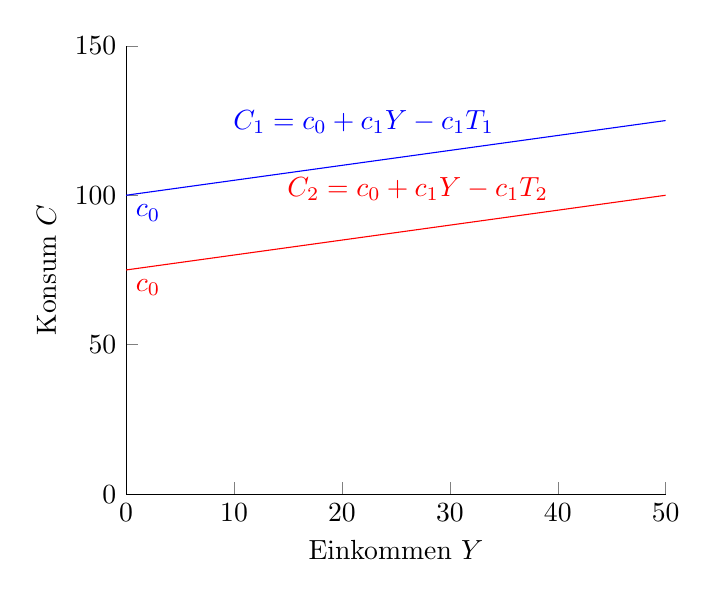
\begin{tikzpicture}
  \begin{axis}[ 
    xmin=0,   xmax=50,
    ymin=0,   ymax=150,
    domain=0:50,
    axis x line*=bottom,
    axis y line*=left,
    xlabel=$\text{Einkommen }Y$,
    ylabel={$\text{Konsum }C$}
  ] 
    \addplot +[mark=none] {100 + 0.5 * x}node[above left,pos=0.7] {$C_1 = c_0 + c_1 Y - c_1 T_1$} node[below right, pos=0] {$c_0$}; 
    \addplot +[mark=none] {75 + 0.5 * x}node[above left,pos=0.8] {$C_2 = c_0 + c_1 Y - c_1 T_2$} node[below right, pos=0] {$c_0$}; 
  \end{axis}
\end{tikzpicture}
\item Investitionen (I)
\label{sec:orgb53fbb6}
\newline
Investitionen werden in diesem Modell als gegeben betrachtet, d.h als exogen angenommen. Gekennzeichnet wird dies durch einen Strich über der Variable: \(I = \bar{I}\) .
\item Staatsausgaben (G) und Steuern (T)
\label{sec:org3bb7986}
\newline
Basierend auf dem Regierungsprogramm ergibt sich ein bestimmtes Ausmaß an Staatsausgaben und Steuern, in diesem Sinn sind beide ebenfalls exogen: \(G = \bar{G}\) und \(T = \bar{T}\) (T sind Steuern minus Transfers).

Laut Regierungsprogramm sind die Staatsausgaben durch Steuern finanziert, daher nehmen wir an, dass der Haushalt in der Ausgangssituation ausgeglichen ist: \(G = T\) .
Werden Staatsausgaben oder Steuern verändert, um die gesamtwirtschaftliche Nachfrage zu beeinflussen, spricht man von Fiskalpolitik
\end{enumerate}
\subsubsection{Gleichgewicht auf dem Gütermarkt (Bestimmung der Produktion)}
\label{sec:orga137012}
Ein \textbf{Gleichgewicht auf dem Gütermarkt} stellt sich dann ein, wenn die \textbf{Güterproduktion Y} der \textbf{Güternachfrage Z} entspricht: \(Y = Z\). Dies ist eine Gleichgewichtsbedingung. Somit gilt (für \(X=IM=0\)):
\begin{equation*}
\begin{aligned}
Y = c_0 + c_1*(Y-\bar{T})+\bar{I}+\bar{G}
\end{aligned}
\end{equation*}
Im Gleichgewicht entspricht die Produktion Y (linke Seite) der Nachfrage (rechte Seite). Da Nachfrage < Produktionspotential, können die nachgefragten Güter auch produziert werden. Es gibt folgende Zusammenhänge:
\begin{itemize}
\item die Nachfrage (ergo dann = die Produktion, da Nachfrage in diesem Modell entscheidend ist) hängt ihrerseits vom Einkommen Y ab
\item das Einkommen Y wiederum ist gleich der Produktion (bzw dem Produktionswert) Y (weil jeder durch Produktion eingenommene Euro, als Einkommen eingenommen wurde)
\item somit wird dasselbe Symbol Y sowohl für die Produktion als auch fuer das Einkommen verwendet
\end{itemize}

Die Gleichgewichtsbedingung spiegelt die zentrale Modellannahme wieder, dass die Produktion nur durch die Nachfrage bestimmt wird (nachfrageseitiges Modell).

\subsubsection{Gleichungen des Gütermarktmodells}
\label{sec:org377af73}
Das Modell besteht aus folgenden Arten von Gleichungen:
\begin{itemize}
\item Definitionsgleichungen, hier: \(Z \equiv C + I + G\) und \(Y_v \equiv Y - T\)
\item Verhaltensgleichungen, hier: \(C= c_0 + c_1*(Y-T)\)
\item Gleichgewichtsbedingung, hier: \(Y=Z\) (Produktion = Güternachfrage)
\end{itemize}

Die Modellgleichungen enthalten:
\begin{itemize}
\item endogene Variablen, hier: C, Y, Z
\item exogene Variablen, hier: \(\bar{I}, \bar{G}, \bar{T}\)
\item Parameter, hier: c\(_{\text{0}}\), c\(_{\text{1}}\)
\end{itemize}

In Modellen analysieren wir meist nur gleichgewichtige Situationen.

Die Gleichgewichtsbedingung kann unter Einführung zwei neuer Begriffe wiefolgt umformuliert werden:

\begin{equation*}
\begin{aligned}
Y = c_0 + c_1*(Y-\bar{T})+\bar{I}+\bar{G}\\
Y = c_0 + c_1*Y - c_1 * \bar{T}+\bar{I}+\bar{G} & \qquad |-(c_1*Y) \nonumber\\
Y - c_1 * Y = c_0 - c_1 * \bar{T}+\bar{I}+\bar{G}\\
(1 - c_1)* Y = c_0 - c_1 * \bar{T}+\bar{I}+\bar{G}  & \qquad |:(1-c_1) \nonumber\\
Y = \frac{c_0 - c_1 * \bar{T}+\bar{I}+\bar{G}}{1-c_1} & \qquad | \text{aus Bruch vorziehen}\\
Y = \frac{1}{1-c_1}*[c_0 - c_1 * \bar{T}+\bar{I}+\bar{G}]
\end{aligned}
\end{equation*}
\begin{itemize}
\item \(\frac{1}{1-c_1}\) = Multiplikator
\item \([c_0 - c_1 * \bar{T}+\bar{I}+\bar{G}]\) = autonome Ausgaben
\end{itemize}

\subsubsection{Graphische Analyse}
\label{sec:org1c9ef00}
\(\rightarrow\) Siehe handschriftliches Blatt

\subsubsection{Der Multiplikatoreffekt}
\label{sec:org683bb5c}
Der Multiplikator ist die Summe sukzessiver Anstiege der Produktion, die aus einem Anstieg der Nachfrage resultieren

Beispielsweise eine Erhöhung der autonomen Staatsausgaben: \(\Delta Y_1 = \Delta \bar{G}\)

\begin{enumerate}
\item Folgerunde: Erhöhung des Konsums: \(\Delta Y_2 = \Delta C_1 = c_1 * \Delta Y_1 = c_1*\Delta \bar{G}\)

\item Folgerunde: Erhöhung des Konsums: \(\Delta Y_3 = \Delta C_2 = c_{1}^{2} * \Delta Y_2 = c_{1}^{2} *\Delta \bar{G}\)
\end{enumerate}

..es folgen weitere Runden, insgesamt ergibt sich: Anstoß + induzierte Konsumnachfrage

Steigt die autonome Nachfrage um 1 Mio., dann ergibt sich nach \(n\) Runden eine Erhöhung der Produktion um 1 Mio. \emph{multipliziert} mit der folgenden Summe: \(1+ c_1 + c_{1}^{2} + ... + c_{1}^{n}\). Das ist eine geometrische Reihe für die bei \(c_1<1\) gilt:

\begin{equation*}
\begin{aligned}
\lim\limits_{n \to \infty}1+ c_1 + c_{1}^{2} + c_{1}^{3} + ... + c_{1}^{n} = \frac{1}{1-c_1}\
\end{aligned}
\end{equation*}

\subsubsection{Die verbale Analyse}
\label{sec:org686d8a9}
Kurzfristig (in der kurzen Frist) wird die Produktion von der Nachfrage bestimmt
\begin{itemize}
\item die Nachfrage hängt ihrerseitz vom Einkommen ab Z(Y)
\end{itemize}

Ein Anstieg der Nachfrage (zB Anstieg der Staatsausgaben) führt zu Anstieg der Produktion und zu einem entsprechenden Anstieg des Einkommens
\begin{itemize}
\item diese Einkommenserhöhung induziert einen weiteren Anstieg der Nachfrage \(\rightarrow\) dies führt wiederum zu einer weiteren Produktionssteigerung usw.
\end{itemize}

Im Endergebnis fällt der Anstieg weit größer aus als die ursprüngliche Verschiebung der Nachfrage und zwar genau um den Faktor, der dem Multiplikator entspricht

Wie lange dauert es bis dieser Anpassungsprozess abgeschlossen ist?
Nach einem Anstieg der Konsumausgaben wird nicht sofort das neue Gleichgewicht erreicht. Es findet vielmehr ein allmählicher Prozess der Anpassung statt.
\begin{itemize}
\item Geschwindigkeit hängt davon ab wie schnell die Firmen auf die neue Situation mit Produktionsanpassungen reagieren
\end{itemize}

Die formale Beschreibung dieser Anpassung der Produktion über die Zeit wird als \textbf{Dynamik} der Anpassung bezeichnet.

\subsubsection{Investition gleich Ersparnis}
\label{sec:orgc8dc60e}
Rest des verfügbaren Einkommens, der nicht für Konsum ausgegeben wird, wird gespart:

\begin{itemize}
\item Definitionsgleichung, hier: \(S = Y_v - C\)
\item Verhaltensgleichung (keynesianische Sparfunktion), hier:
\end{itemize}
\begin{equation*}
\begin{aligned}
S = Y - T - c_0 - c_1(Y-T) \\
= -c_0 + (1-c_1)*(Y-T)
= -c_0 + (1-c_1) * Y_v
\end{aligned}
\end{equation*}
\begin{itemize}
\item Gleichgewichtsbedingung, hier:
\end{itemize}
\begin{equation*}
\begin{aligned}
Y = C + I + G
Y - T -C = I + G - T
S = I + G - T
I = S + (G-T)
\end{aligned}
\end{equation*}
S = Ersparnis privater Haushalte, (T - G) = Ersparnis des Staates

\subsubsection{Ist die Regierung allmächtig? Eine Warnung}
\label{sec:orgdb61413}
\begin{enumerate}
\item Kann die Regierung Einfluss nehmen?
\label{sec:orgf6e2a43}

Fiskalpolitik = Teil der Finanzpolitik, der dem Stabilisierungsziel gewidmet ist; die Variation von Staatsausgaben bzw -einnahmen zur Beeinflussung der aggregierten Güternachfrage
\begin{center}
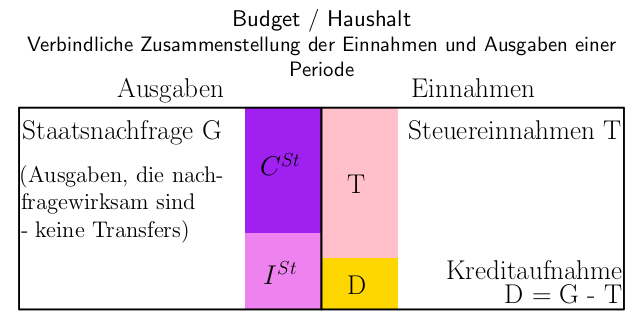
\includegraphics[width=.9\linewidth]{./budgethaushalt.png}
\end{center}

\(Y = \frac{1}{1-c_1}*[c_0-c_1\textcolor{magenta}{\bar{T}} + \bar{I} + \textcolor{magenta}{\bar{G}}]\)

direkte Maßnahmen:
\begin{itemize}
\item Änderung der Staatsausgaben
\item Änderung der Steuern bzw der Transfers
\end{itemize}

indirekte Maßnahmen:
\begin{itemize}
\item Investitionszulagen
\item Abschreibungsvergünstigungen
\end{itemize}

\item Wer ist für Fiskalpolitik verantwortlich?
\label{sec:org4ee1501}

Staat = Institution mit hoheitlicher Gewalt, d.h. Staat ist legitimiert \& fähig Zwangsmaßnahmen auszuüben

Staatsquote = \(\frac{\text{Ausgaben der öffentl. Haushalte}}{\text{Bruttoinlandsprodukt}}\) in Prozent
\item Kreditfinanzierte Erhöhung der Staatsausgaben
\label{sec:org795092d}

Eine Erhöhung der Staatsausgaben G erhöht die Nachfrage (\(\rightarrow\) Z-Kurve verschiebt sich nach oben), sodass Einkommen steigt und zwar gemäß dem Multiplikator um \(\frac{\delta Y}{\delta G} = \frac{1}{1-c_1}\).

Da die zusätzlichen Ausgaben kreditfinanziert werden, wird die staatliche Ersparnis (T - G) kleiner. Dies wird aber durch die private Ersparnis S ausgeglichen, die mit dem Einkommen ansteigt.

Da die erhöhten Staatsausgaben kreditfinanziert werden, vergrößert sich der Schuldenstand des Staates (nicht in unserem Modell enthalten!).
\item Steuerfinanzierte Erhöhung der Staatsausgaben
\label{sec:org4bb2e71}

Eine Erhöhung der Staatsausgaben G wird durch eine gleichzeitige Erhöhung der Steuern T finanziert:
\begin{equation*}
\begin{aligned}
Y = \frac{1}{1-c_1}*[c_0-c_1*\bar{T}+\bar{I}+\bar{G}]\\
Y = \frac{1}{1-c_1}*[c_0+\bar{I}+(1 - c_1)*\bar{G}]
\end{aligned}
\end{equation*}
Auch in der neuen Situation gilt G = T und damit bei steuerfinanzierten Änderungen von G: \(\frac{\delta Y}{\delta G} = \frac{1-c_1}{1-c_1} = 1\).
Der Multiplikator ist somit lediglich 1 und damit kleiner als bei kreditfinanzierten Staatsausgaben. Das ergibt sich auch bei separater Betrachtung der Multiplikatoren:
\begin{equation*}
\begin{aligned}
{\underbrace{\textstyle \frac{1}{1-c_1}}_{\mathclap{\text{ Staatsausgabenmultiplikator }}}} 
+
{\overbrace{\textstyle \frac{-c_1}{1-c_1}}^{\mathclap{\text{ Steuermultiplikator }}}}
=
1
\end{aligned}
\end{equation*}

\item Automatische Stabilisatoren
\label{sec:org6c748d6}

Idee: Konjunkturelle Schwankungen der Steuereinnahmen stabilisieren Nachfrage \(Z = c_0 + c_1 *(Y-T)+\bar{I}+\bar{G}\). Steuern (und Transfers) hängen endogen vom Einkommen ab: \(T= t*Y\), mit \(t=\text{Steuersatz} < 1\)

\begin{equation*}
\begin{aligned}
Y = Z = c_0 + c_1- c_1  t Y + \bar{I} + \bar{G} & \qquad |+(c_1*t*Y),|-c_1 \nonumber\\
Y - c_1 + c_1*t*Y = c_0 + \bar{I} + \bar{G}\\
Y (1-c_1+c_1t) = c_0 + \bar{O} + \bar{G}\\
Y = \frac{1}{1-c_1+c_1t}*[c_0+\bar{I}+\bar{G}]
\end{aligned}
\end{equation*}

Der Multiplikator wird kleiner. Bei exogenen Schocks in \(\bar{I}\) oder c\(_{\text{o}}\) fallen Schwankungen geringer aus.

\item Probleme bei Umsetzung direkter Nachfragesteuerung
\label{sec:orgdae81f4}

\begin{itemize}
\item Staatsausgaben oder Steuern rasch zu ändern ist nahezu unmöglich
\item aufgrund komplexer Prozesse sind Auswirkungen auf Konsum, Investitionen, Importe etc. nur mit großer Unsicherheit zu prognostizieren
\item Erwartungen spielen eine große Rolle
\item empirisch ermittelte Multiplikatoren sind viel kleiner als im Modell und teilweise sogar < 1
\item das Ziel eines bestimmten Produktionsniveaus kann unerwünschte Nebenwirkungen nach sich ziehen (zB Preissteigerungen)
\item ein hohes Budgetdefizit \& hohe Staatsverschuldung kann langfristig schädliche Effekte auslösen
\end{itemize}
\end{enumerate}

\subsection{Geld- und Finanzmärkte}
\label{sec:org1f5b2a8}
In diesem Kapitel geht es um das \textbf{Gleichgewicht} auf \textbf{Geld-} und \textbf{Finanzmärkten} und die \textbf{Bestimmung des Zinssatzes}.

\textbf{Geld} kann für Transaktionen (zB Kauf/Verkauf) verwendet werden. Es gibt zwei Arten von Geld:
\begin{itemize}
\item Bargeld (Münzen und Banknoten)
\item Sichtguthaben (Girokonten)
\end{itemize}

Geld kann auch zur Wertaufbewahrung verwendet werden. Da es aber keine Zinsen bringt, werden meist andere Formen der Wertaufbewahrung vorgezogen.

\textbf{Festverzinsliche Wertpapiere} (Bonds) bringen einen positiven Zinssatz i, können aber nicht für Transaktionen verwendet werden.

\textbf{Semantische Fallen:} Geld, Einkommen und Vermögen
\begin{itemize}
\item Einkommen besteht aus der Arbeitsvergütung \& Kapitalerträgen in Form von Zinsen \& Dividenden.
\begin{itemize}
\item wird in Einheiten pro Zeiteinheit ausgedrückt, es handelt sich also um eine Stromgröße
\end{itemize}
\item Ersparnis ist der Teil des Einkommens nach Abzug der Steuern, der nicht ausgegeben wird
\begin{itemize}
\item ebenfalls eine Stromgröße
\end{itemize}
\item Finanzvermögen (oder einfach Vermögen) ist Wert aller Finanzanlagen abzüglich aller Verbindlichkeiten
\begin{itemize}
\item Bestand an Vermögen zu einem gegebenen Zeitpunkt, also eine Bestandsgröße
\end{itemize}
\item Finanzanlagen, die man direkt zum Kauf von Gütern einsetzen kann, werden Geld genannt
\begin{itemize}
\item Geld beinhaltet Bargeld \& Buchgeld (Sichteinlagen)
\item ist auch eine Bestandsgröße
\end{itemize}
\item unter Investitionen verstehen Ökonomen den Kauf von neuen Anlagegütern (Maschinen, Fabriken, Bürogebäude), der Kauf von Aktien oder anderer Finanzanlagen wird dagegen als Finanzinvestition bezeichnet
\end{itemize}

Das Finanzvermögen W der Haushalte setzt sich zusammen aus Geldvermögen und Bonds. Geld wird i.d.R durch das Symbol M gekennzeichnet, Bonds(B) ist der Bestand an festverzinslichen Wertpapieren. Sie habenn den Preis p\(_{\text{B}}\) .
\begin{equation*}
\begin{aligned}
W = M + p_B * B
\end{aligned}
\end{equation*}
Haushalte haben darüber zu entscheiden, welchen Teil ihres Vermögens sie in Form von Geld und welchen in Form von Bonds halten. Geld hat den Vorteil der Liquidität, Bonds den eines Zinsertrages. Die Aufteilung ist abhängig von Transaktionsvolumen und -häufigkeit, sowie dem Zinssatz auf Wertpapiere
\subsubsection{Die Geldnachfrage}
\label{sec:org425ee29}
Die Geldnachfrage M\(^{\text{d}}\)\ldots{}
\begin{itemize}
\item \ldots{}steigt proportional mit dem Nominaleinkommen (\(PY\))
\item \ldots{}hängt negativ vom Zinssatz i ab (wobei L(i) eine Funktion des Zinssatzes ist)
\end{itemize}
\begin{equation*}
\begin{aligned}
M^d = PY*L(i)
\end{aligned}
\end{equation*}

\textbf{Die Ableitung der Geldnachfrage}\\
Für ein gegebenenes Nominaleinkommen \(P_1 Y_1\) erhöht ein niedriger Zinssatz die Geldnachfrage. 
Mit steigendem Zinsatz geht die Liquiditätspräferenz (Präferes für "Flüssiges" also Geld) und damit auch die Geldnachfrage zurück. Screenshot 71

Bei jedem gegebenen Zinssatz verschiebt sich eine Erhöhung des Nominaleinkommens die Geldnachfrage nach rechts: Screenshot 72

\textbf{Geldnachfrage \& Zinsen - Empirische Evidenz}\\
Wie gut bildet die Geldnachfragegleichung die Realität ab?
\(M^d = PY * L(i)\) \(\rightarrow\) teile beide Seiten durch \(PY\): \(\frac{M^d}{PY}=L(i)\)

\(L(i)\) = \textbf{Kassenhaltungskoeffizient} \(\equiv \frac{\text{Geldhaltung}}{\text{Nominaleinkommen}}\)
\begin{itemize}
\item wenn der Zinssatz hoch ist, dann sollte \(L(i)\) niedrig sein
\item wenn der Zinssatz niedrig ist, dann sollte \(L(i)\) hoch sein
\end{itemize}

Kehrwert: \(\frac{1}{L(i)}\) = \textbf{Umlaufgeschwindigkeit des Geldes}

\subsubsection{Gleichgewicht auf dem Geldmarkt}
\label{sec:orgb395d10}
Wir betrachten in diesem Modell zunächst eine Wirtschaft, in der es \textbf{keine Geschäftsbanken} gibt. Es gibt dhaer \textbf{kein Buchgeld}. Geld ist gleichbedeutend mit \textbf{Bargeld}. Angenommen die Zentralbank entscheidet sich, eine Geldmenge in Höhe von \(\bar{M}\) zur Verfügung zu stellen, so dass das Geldangebot \(M^s = \bar{M}\) ist.
So stellt sich ein Gleichgewicht auf dem Geldmarkt dann ein, wenn das Geldangebot gleich der Geldnachfrage ist:
\begin{equation*}
\begin{aligned}
M^s = \bar{M}
\bar{M} = PY * L(i)
\end{aligned}
\end{equation*}

\begin{enumerate}
\item Geldnachfrage, Geldangebot \& Gleichgewichtszinssatz
\label{sec:org8f75da6}
Die Bestimmung des Zinssatzes: Der Zinssatz pendelt sich im Gleichgewicht so ein, dass die (zinsabhängige) Geldnachfrage dem gegebenen Geldangebot entspricht. Screenshot 76

Die Auswirkungen eines \emph{höheren Nominaleinkommens} auf den Gleichgewichtszins: Mit steigendem Nominaleinkommen verschiebt sich die Geldnachfragekurve nach rechts, der Gleichgewichtszins steigt. Screenshot 77

Die Auswirkungen eines \emph{höheren Geldangebots} auf den Gleichgewichtszins: Eine Zunahme des Geldangebots verschiebt die Geldangebotskurve nach rechts, der Gleichgewichtszins sinkt: Screenshot 78
\end{enumerate}

\subsubsection{Geldpolitik}
\label{sec:org84d69bc}
Wie kann die Zentralbank das Geldangebot verändern und was geschieht, wenn sie es verändert?
\begin{itemize}
\item Geldmengenerhöhung = Zentralbank kauft Wertpapiere und bezahlt mit neu geschöpftem Geld
\item Geldmengenverringerung = Zentralbank verkauft Wertpapiere und entzieht dem Wirschaftskreislauf Geld
\end{itemize}

Derartige Operationen werden \textbf{Offernmarktgeschäfte} genannt, da sie am "offenen Markt" für Wertpapiere durchgeführt werden.
In moderenen Volkswirtschaften steuern alle Zentralbanken die Geldmenge über solche Offenmarktgeschäfte.

Die Bilanz der Zentralbank: Screenshot 80

Die Aktiva der Zentralbank bestehen aus den Wertpapieren, die sie hält. Ihre Passiva entsprechen der Geldmenge.

In einer \emph{expansiven Offenmarktoperation} kauft die Zentralbank bspw Wertpapiere im Wert von 1 Mio.\texteuro{} und zahlt mit eigenem Bargeld. Sie erhöht so das Geldangebot um 1 Mio\texteuro{}:
Screenshot 81

\(\rightarrow\) Wirkung: Preis für Wertpapiere steigt, Zinssatz sinkt

\begin{enumerate}
\item Beispiel zum Zusammenhang zwischen Zins und Wertpapierpreis
\label{sec:orgc02ab61}

\begin{itemize}
\item Wertpapier B mit Auszahlung(swert) von 100 Euro (=Nennwert) im nächsten Jahr
\item Laufzeit ein Jahr
\item i: Zinssatz für Laufzeit von einem Jahr
\end{itemize}

Wie bestimmt sich der Preis \$P\(_{\text{B}}\) \$ des Wertpapiers heute?

Für eine Anleihe mit einjähriger Laufzeit:

\begin{equation*}
\begin{aligned}
P_B = \frac{100}{1+i} \rightarrow P_B*(1+i)=100
\end{aligned}
\end{equation*}

\begin{itemize}
\item für \(i=5.3\%\) gilt: \(P_B = 95\)
\item für \(i=11.11\%\) gilt: \(P_B = 90\)
\end{itemize}

Warum, was steckt dahinter?

Dahinter steck folgendes Arbitragekalkül:
\begin{itemize}
\item Eine Alternativanlage vom Betrag X Euro heute zum Zins i bringt mir im nächsten Jahr den Ertrag \(X*(1+i)\) Euro
\item Will ich einen Ertrag von \(X*(1+i)=100\), muss ich also heute anlegen: \(X=\frac{100}{1+i}\)
\item falls \(P_B > X\) würde Niemand das Papier B kaufen (Preis wäre zu hoch, er müsste auf \(P_B = X\) sinken)
\item falls \(P_B < X\) würden alle das Papier B kaufen (dies treibt den Preis au \(P_B = X\) hoch)
\end{itemize}

Betrachtung eines \emph{"alten"} Wertpapiers, das im nächsten Jahr eine Gesamtauszahlung von 100 Euro verspricht. Wie hoch ist der Kurs des Papiers P\(_{\text{B}}\) heute?

\(\rightarrow\) Vergleiche mit der Rendite von neuen, \textbf{einjährigen} Papieren

Bsp: aktueller Zins für einjährige Papiere bei \(i=25\%\).
Wer in einem Jahr eine Auszahlung von 100 Euro erwünscht, muss heute \(\frac{100\text{Euro}}{1.25}=80\) Euro anlegen.

\textbf{Effektivrendite:} \(i=0.25 \rightarrow 1 + i = 100\)

\textbf{Kurs:} \(P_B = \frac{100}{1+i} = \frac{100}{1.25} = 80\)

\begin{itemize}
\item solange \((1+i)*P_B > 100\) kauft jeder lieber neue Papiere \& es wäre besser, das "alte" Wertpapier zu verkaufen
\item falls \((1+i)*P_B < 100\) kauft jeder lieber das "alte" Wertpapier, schon für \(P_B < 80\) bekäme man im nächsten Jahr 100 Euro
\end{itemize}

\emph{Anderes Beispiel:}\\
Gesamtauszahlung meines Papiers in einem Jahr: 100 Euro\\
Angenommen der Zins steigt heute auf \(i=50\%\), wie wirkt sich das auf den Kurs meines Papiers P\(_{\text{B}}\) aus?

\(\rightarrow\) Der Kurs muss so stark fallen, dass die Effektivrendite auf 50\% steigt! (umgekehrt würde der Kurs bei einer Zinssenkung steigen)

Kurs bei \(i=50\%\): \(P_B=\frac{100}{1.5}\) \(=66.\frac{1}{3}\)
Kurs bei \(i=25\%\): \(P_B=\frac{100}{1.25}\) \(=80\)
Kurs bei \(i=10\%\): \(P_B=\frac{100}{1.10}\) \(=90.91\)
Kurs bei \(i=0\%\): \(P_B=\frac{100}{1}\) \(=100\)

\textbf{Fazit zum Zusammenhang zwischen Zins und Wertpapierpreis}
\begin{itemize}
\item es besteht eine inverse Beziehung zwischen Wertpapierpreis \& Zins \(\rightarrow\) wenn der Wertpapierpreis sinkt (steigt), steigt (sinkt) die Rendite
\item je länger die Laufzeit, desto stärker der Effekt auf die Kurse
\item \textbf{Beachte:} allein schon Zinsänderungen, die nur erwartet (antizipiert) werden, wirken sich bereits unmittelbar heute auf die Kurse aus
\end{itemize}

\textbf{Wirkung von Offenmarktoperationen:}
\begin{itemize}
\item expansive Offenmarktoperation: Erhöhung der Geldmenge, Zinssenkung
\begin{itemize}
\item \(\rightarrow\) Zentralbank kauft Wertpapiere und gibt dafür Geld raus
\item Wirkung: Zinssatz sinkt, da \textbf{Nachfrage} nach Wertpapieren steigt (P\(_{\text{B}\uparrow}\))
\end{itemize}
\item kontraktive Offenmarktoperation: Verringerung der Geldmenge, Zinserhöhung
\begin{itemize}
\item \(\rightarrow\) Zentralbank verkauft Wertpapiere \& erhält dafür Geld
\item Wirkung: Zinssatz steigt, da \textbf{Angebot} an Wertpapieren steigt (P\(_{\text{b}}\) \(\downarrow\))
\end{itemize}
\end{itemize}

\textbf{Zusammenfassung Geldpolitik und Offenmarktgeschäfte}
\begin{itemize}
\item der Zinssatz wird durch Gleichheit von Geldnachfrage \& Geldangebot bestimmt
\item die Zentralbank kann den Zinssatz beeinflussen, indem sie das Geldangebot verändert
\item die Zentralbank verändert das Geldangebot mittels Offenmarktgeschäften
\item der Ankauf von Wertpapieren erhöht das Geldangebot und reduziert den Zinssatz
\item der Verkauf von Wertpapieren senkt das Geldangebot und erhöht den Zinssatz
\end{itemize}
\end{enumerate}
\subsubsection{Zweite Bestimmung des Gleichgewichts}
\label{sec:org602a700}
Wir heben jetzt die Beschränkung auf, dass es keine Geschäftsbanken gibt und das Geld nur aus Bargeld besteht. Durch die Existenz von Geschäftsbanken wird die Kontrolle der Geldmenge schwieriger, da Banken durch Kreditgewährung die Höhe des Buchgeldes beeinflussen.

Es ist jetzt sinnvoll zu unterscheiden:
\begin{itemize}
\item \textbf{Zentralbankgeld} H = Bargeld und Sichtguthaben bei der Zentralbank (H = high powered money)
\item Geld M: Bargeld und Sichtguthaben bei Geschäftsbanken, die von Nichtbanken (Haushälte, produzierende Unternehmen, Staat) gehalten werden (M = money)
\end{itemize}

\textbf{Was Banken machen}\\
Banken erhalten Einlagen von Privatpersonen \& Unternehmen und kaufen damit festverzinsliche Wertpapiere oder Aktien oder vergeben Kredite an andere Privatpersonen o Unternehmen. Einen Teil der eingezahlten Einlagen behalten die Geschäftsbanken als Reserve (zum Teil als Bargeld, zum Teil auf Konten, die die Geschäftsbanken bei der Zentralbank haben).

Gründe: Einzahlungen und Auszahlungen der Anleger sind nicht gleich groß, die Geschäftsbank muss immer eine gewisse Menge an Bargeld bereithalten, \ldots{}
\begin{itemize}
\item \ldots{} um Schulden ggü anderen Banken zu decken
\item \ldots{} um die gesetzlichen Mindestreserveverpflichtungen zu erfüllen
\end{itemize}

Kredite entsprechen ungefähr 70\% des Vermögens von Geschäftsbanken nach Abzug der Reservepflicht. Die restlichen 30\% entfallen auf Wertpapiere.
Das Vermögen der Zentralbank besteht aus den von ihr gehaltenen Wertpapieren. Die Verbindlichkeiten der Zentralbank bestehen aus dem von ihr geschaffenen Geld (\textbf{Zentralbankgeld}). Neu ist, dass nicht das gesamte Zentralbankgeld in Form von Bargeld von Nicht-Banken gehalten wird. Ein Teil davon wird als Reserve von den Geschäftsbanken gehalten.

Bilanz von Zentralbank und Geschäftsbanken:
Screenshot 92

Geldangebot = verfügbare Geldmenge = \({\overbrace{\textstyle \text{Münzen \& Noten}}^{\mathclap{\text{ Zentralbankgeld H }}}}\) \(+ {\underbrace{\textstyle \text{Sichteinlagen}}_{\mathclap{\text{enstehen durch Einzahlung von Zentralbankgeld}}}}\)

\textbf{Buchgeldentstehung im System mit 100-\%iger Reservehaltung}:\\
Zentralbank kauft Wertpapier von Person A \& zahlt mit Noten im Wert von 100 \(\rightarrow\) Geldmenge M = 100 (Noten) \(\rightarrow\) A zahlt Noten auf Girokonto ein, Bank hinterlegt sie bei der ZB als Reserve
Screenshot 94
Banken haben hier keinen Einfluss auf das Geldangebot

\textbf{Buchgeldentstehung bei partieller Reservehaltung}:\\
Sachverhalt wie vorher, aber Reservesatz \(r=0.1\)(10\%)

Screenshot 95 1

Bank verwendet die Überschussreserve (Kasse) zur Kreditvergabe. Der Kreditnehmer B zahlt mit den erhaltenen
Noten eine Rechnung von C , die dieser bei Bank 2 einzahlt. Bank 2 verwendet Überschussreserve ebenfalls zur
Kreditvergabe, \ldots{}

Screenshot 95 2

Dieser Prozess kann sich fortsetzen = \textbf{Geldschöpfungsprozess}

Ausgangspunkt: Zentralbank (Bargeld/Sichteinlage bei Zentralbank)
Screenshot 96

\textbf{Die Nachfrage nach Geld, Reserven und Zentralbankgeld}\\
Nichtbanken fragen Geld nach: \(M^d = PY * L(i)\)

Der Anteil c soll als Bargeld gehalten werden: \(CU^d = cM^d\)
und (1-c) als Sichtguthaben: \(D^d=(1-c)M^d\).

Die Geschäftsbanken halten den Anteil \(\theta\) der Sicht-Guthaben als Reserve bei der Zentralbank: \(R^d = \theta D= \theta (1-c)M^d\).

Als Nachfrage nach Zentralbank ergibt sich:
\begin{equation*}
\begin{aligned}
H^d = C U^d + R\\
= c M^d + \theta(1-c)M^d\\
= (c + \theta (1-c))*M^d\\
= (c + \theta (1-c))*PY * L(i)
\end{aligned}
\end{equation*}

\textbf{Angebot, Nachfrage und Zinsbestimmung}\\
Die Zentralbank stellt ein Geldangebot in Höhe \(\bar{H}\) bereit:
\begin{equation*}
\begin{aligned}
H^s = \bar{H}
\end{aligned}
\end{equation*}
Im Gleichgewicht: Angebot an Zentralbankgeld = Nachfrage nach Zentralbankgeld 
\begin{equation*}
\begin{aligned}
H^s = H^d\\
\bar{H} = (c+\theta (1-c))PY * L(i)
\end{aligned}
\end{equation*}
Screenshot 99

\subsubsection{Alternativer Ansatz}
\label{sec:org192275a}
Statt Angebot und Nachfrage nach Zentralbankgeld zu analysieren, kann man alternativ Angebot \& Nachfrage nach Reserven betrachten:
\begin{equation*}
\begin{aligned}
{\underbrace{\textstyle \bar{H} - CU^d}_{\mathclap{\text{ Angebot an Reserven}}}} = {\overbrace{\textstyle R^d}^{\mathclap{\text{ Nachfrage nach Reserven}}}}
\end{aligned}
\end{equation*}

Dies ist von Interesse, weil die Geschäftsbanken täglich auf einem Markt für Reserven - dem \textbf{Tagesgeldmarkt} - handeln.
\begin{itemize}
\item Banken deren Reserven höher sind als geplant, bieten an
\item Banken deren Reserven niedriger sind als geplant, fragen nach
\end{itemize}

Gleichgewicht: \(\bar{H} = (c + \theta(1-c)) PY * L(i)\)

Diese Gleichgewichtsbedingung kann umgestellt werden zu
\begin{equation*}
\begin{aligned}
{\underbrace{\textstyle \frac{1}{c+\theta(1-c)} \bar{H}}_{\mathclap{\text{gesamtes Geldangebot}}}} = {\overbrace{\textstyle PY*L(i)}^{\mathclap{\text{ gesamte Geldnachfrage}}}}
\end{aligned}
\end{equation*}

Der Term \(\frac{1}{c+\theta(1-c)}\) heißt \textbf{Geldschöpfungsmultiplikator}
\begin{itemize}
\item der Multiplikator ist größer als 1, denn \(0<c\), \(\theta<1\) \(\rightarrow\) der Mindestreservesatz \(\theta\) beträgt mindestens 1\%.
\item Spezialfälle:
\begin{itemize}
\item c = 1: Nur Bargeldhaltung \(\rightarrow\) Multiplikator = 1, d.h die gesamte Geldmenge entspricht der Zentralbankgeldmenge
\item c = 0: keine Bargeldhaltung \(\rightarrow\) Multiplikator = \(\frac{1}{\theta}\) \(\rightarrow\) bei \(\theta\) = 0.01 wird die gesamte Geldmenge zum 100-fachen von \(\bar{H}\)
\end{itemize}
\end{itemize}

\begin{enumerate}
\item Vergleich Zinsbestimmung I und II
\label{sec:orged99511}
Zinsbestimmung I:
\begin{itemize}
\item Gleichgewicht \(\bar{M} = PY * L(i)\)
\end{itemize}

Zinsbestimmung II:
\begin{itemize}
\item Gleichgewicht \(\frac{1}{c+\theta (1-c)}\bar{H} = PY * L(i)\) (\(\bar{H}\) wird auch Geldbasis genannt)
\end{itemize}

Der Unterschied liegt auf der Angebotsseite:
\begin{itemize}
\item Bestimmung II macht deutlich, dass die monetäre Steuerung über die Zentralbankgeldmenge erfolgt
\item Bestimmung II macht auch deutlich, dass die Zentralbank die Geldmenge nicht unabhängig festsetzen kann, da c von den Nichtbanken und \(\theta\) von den Geschäftsbanken bestimmt wird
\end{itemize}
\end{enumerate}
\subsection{Das IS-LM Modell}
\label{sec:orgf0d8a91}
In den vorhergehenden Kapiteln wurde der Gütermarkt und der Geld- und Finanzmarkt betrachtet. Es wurde isoliert die Höhe der Produktion und des Zinssatzes bestimmt.

Jetzt soll das Zusammenspiel dieser Märkte untersucht werden. Zunächst werden alternative Gütermarktgleichgewichte (IS-Kurve) und danach alternative Geldmarktgleichgewichte (LM-Kurve) hergeleitet.

Produktion und Zinssatz werden dann simultan bestimmt und es wird der Einfluss von Geld- und Fiskalpolitik untersucht.

\subsubsection{Gütermarkt und IS-Gleichung}
\label{sec:org2a7f663}
\begin{enumerate}
\item Investition, Absatz und Zinssatz
\label{sec:orgb5f975f}

In diesem Kapitel betrachten wir 2 Faktoren, welche die Investitionen beeinflussen:
\begin{itemize}
\item das Absatzniveau (+)
\item der Zinssatz (-)
\end{itemize}
\(\rightarrow\) gemessen durch Y Kreditkostenelement, Alternativrendite und Wertpapierkauf

Investition \(I = I(Y,i)\)
\begin{itemize}
\item \(\frac{\delta I}{\delta Y} > 0\)
\item \(\frac{\delta I}{\delta i} < 0\)
\end{itemize}

Hier wird unterstellt, dass Investitionen vom Nominalzinssatz abhängen und nicht vom Realzinssatz, welcher Preisniveauänderungen berücksichtigt. In der kurzen Frist ist dies plausibel, da das Preisniveau als konstant angenommen wird.

\item Die Bestimmung des Produktionsniveaus
\label{sec:org7f4bc27}

\begin{equation*}
\begin{aligned}
I = I(Y,i)
\end{aligned}
\end{equation*}

Unter Berücksichtigung der obigen Gleichung für die Investitionen erhalten wir als Gleichgewichtsbedingung:
\begin{equation*}
\begin{aligned}
Y = Z \equiv C(Y-\bar{T})+I(Y,i)+\bar{G}
\end{aligned}
\end{equation*}
\(\uparrow\) Einkommensänderungen haben einen positiven Zusammenhang auf/mit \(C(Y-\bar{T})\) und \(I(Y,i)\):
\begin{itemize}
\item es wird unterstellt, dass eine Zunahme des Einkommens um 1\texteuro{} die Nachfrage(C,I) um weniger als 1\texteuro{} erhöht
\item die Produktion ist abhängig von der Nachfrage, die ihrerseits abhängig ist von der Produktion/dem Einkommen
\end{itemize}

Um die Z-Kurve graphish darstellen zu können, müssen wir von einem bestimmten Zinssatz i\(_{\text{1}}\) ausgehen.

Screenshot 112
Die Güternachfrage nimmt mit steigendem Einkommen zu. Im Gleichgewicht muss die Nachfrage dem Einkommen entsprechen.
\begin{itemize}
\item zu beachten: Wir nehmen an, dass die Z-Kurve flacher ist als die 45 Grad Linie
\begin{itemize}
\item Eine Zunahme des Einkommens lässt die Nachfrage nicht im Verhältnis 1:1, sondern weniger ansteigen
\end{itemize}
\end{itemize}

\item Die IS-Kurve
\label{sec:orgd889f84}

Wir haben jetzt die Produktion für den Fall bestimmt, dass der Zinssatz i\(_{\text{1}}\) beträgt.

Ändert sich der Zinssatz, dann ändern sich die Investitionen und damit die Nachfrage. Es ergibt sich ein neues Gleichgewicht.

Leitet man für verschiedene Zinssätze i das resultierende gleichgewichtige Einkommen Y her und trägt diese (Y,i)-Kombinationen in ein Achsenkreuz ein, dann erhält man die IS-Kurve.

\textbf{Ableitung der IS-Kurve} (=die Auswirkungen eines Zinsanstiegs auf das Einkommens)\\
Screenshot 145
\begin{itemize}
\item ein Anstieg des Zinssatzes lässt die Investitionen und damit das Einkommen zurückgehen
\item die Güternachfrage verschiebt sich nach unten
\item es ergibt sich ein neues Gleichgewicht beim niedrigeren Einkommen Y\(_{\text{2}}\)
\end{itemize}

Die IS-Kurve beschreibt alternative Gleichgewichte des Gütermarktes. Mit sinkendem Zinssatz steigen die Investitionen an und damit steigt das Einkommen im Gütermarktgleichgewicht (die IS-Kurve hat deshalb einen fallenden Verlauf)
Screenshot 115

\textbf{Die Steigung der IS-Kurve}\\
Screenshot 116

Ausgangspunkt A: (Y\(_{\text{1}}\), i\(_{\text{1}}\)) \(\rightarrow\) Zinsen sinken auf i\(_{\text{2}}\) 

Argumentationskette:\\
i\(\downarrow\) dann(Zinsreagibilität der Investitionen) I(i) \(\uparrow\) dann(Multiplikatorprozess) Y\(\uparrow\)


Die IS-Kurve ist umso steiler
\begin{itemize}
\item je weniger elastisch die Investitionen auf Zinsänderungen reagieren
\item je kleiner der Multiplikator ist
\item Extremfall wenn I unabhängig von i sind, dann ist IS-Kurve senkrecht
\end{itemize}

\textbf{Verschiebung der IS-Kurve}\\
1.) Wirkung eines Anstiegs der Staatsausgaben von \(\bar{G_1}\) auf \(\bar{G_2}\)

Screenshot 117

Höhere Staatusausgaben G verschieben die IS-Kurve nach rechts. Bei exogen gegebenen Investitionen gemäß Kapitel 3:
\begin{equation*}
\begin{aligned}
Y = \frac{1}{1-c_1}(c_0 + \bar{I} + \bar{G} - c_1 * \bar{T})\\
\Delta Y = \frac{1}{1-c_1}*\Delta\bar{G}
\end{aligned}
\end{equation*}
Der Multiplikatoreffekt ist hier noch größer, da auch die Investitionen mit Y ansteigen.

2.) Wirkung einer Erhöhung der Steuer von \(\bar{T_1}\) auf \(\bar{T_2}\)

Screenshot 118

Höhere Steuern T verschieben die IS-Kurve nach links. Bei exogen gegebenen Investitionen gemäß Kapitel 3:
\begin{equation*}
\begin{aligned}
Y = \frac{1}{1-c_1}(c_0 + \bar{I} + \bar{G} - c_1 * \bar{T})\\
\Delta Y = \frac{-c_1}{1-c_1}*\Delta\bar{T}
\end{aligned}
\end{equation*}
Der Multiplikatoreffekt ist hier noch größer, da auch die Investitionen mit Y sinken.
\end{enumerate}


\subsubsection{Geld- und Finanzmärkte und LM-Gleichung}
\label{sec:orgb801ff2}
\begin{enumerate}
\item Die LM-Kurve
\label{sec:org7985d39}

Im Geldmarktgleichgewicht gilt:
\begin{equation*}
\begin{aligned}
\frac{\bar{m}}{P} = Y * L(i)
\end{aligned}
\end{equation*}
Wir stellen nun folgende Frage: Für welche Kombinationen aus Zins und Einkommen (Y, i) befindet sich der Geldmarkt im Gleichgewicht?

Leitet man für verschiedene Einkommen Y den resultierenden gleichgewichtigen Zinssatz i her und trägt diese (Y,i)-Kombinationen in ein Achsenkreuz ein, so erhält man die LM-Kurve

\textbf{Ableitung der LM-Kurve}\\
Die Auswirkungen einer Erhöhung des Einkommens von Y\(_{\text{1}}\) auf Y\(_{\text{2}}\) auf den Zinssatz:

Screenshot 121

\begin{itemize}
\item mit steigendem Einkommen steigt bei gegebenem Zinssatz die Geldnachfrage
\item die Wirtschaftssubjekte versuchen, Wertpapiere zu verkaufen und das führt zum Sinken des Wertpapierpreises
\item daraufhin muss bei gegebenem Geldangebot im Gleichgewicht der Zinssatz steigen
\end{itemize}

Die LM-Kurve beschreibt alternative Gleichgewichte auf Geld- und Finanzmärkten.

Mit steigendem Einkommen muss der Zinssatz steigen, damit Gleichgewicht auf Geld- und Finanzmärkten herrscht:
Screenshot 122

Die LM-Kurve hat deshalb einen steigenden Verlauf

\textbf{Die Steigung der LM-Kurve}\\
Screenshot 123

Ausgangspunkt A: (Y\(_{\text{1}}\), i\(_{\text{1}}\)) \(\rightarrow\) Einkommen steigt auf Y\(_{\text{2}}\) 

Argumentationskette:\\
Y\(\uparrow\) dann(Zinsreagibilität der Geldnachfrage) M\(^{\text{d}}\) \(\uparrow\) dann i\(\uparrow\)

Umschichtung der Geldnachfrage: Für vermehrte Transaktionen wird mehr Geld gebraucht, das durch Zinssteigerungen dem Spekulationsbereich, in dem Geld als Wertanlage gehalten wird, entzogen wird.

Die LM-Kurve ist umso steiler
\begin{itemize}
\item je kleiner die Geldnachfrage auf Zinsänderungen reagiert
\end{itemize}

\textbf{Anpassungsreaktion der LM-Kurve im Ungleichgewicht}\\
Auf dem Geldmarkt erfolgt die Anpassung über den Zinssatz

\textcolor{violet}{Punkt B}: \(\frac{M}{P} > Y * L(i)\) also ein Überangebot an Geld \(\rightarrow\) Zinsen sinken

\textcolor{magenta}{Punkt C}: \(\frac{M}{P} < Y * L(i)\) also eine Übernachfrage nach Geld \(\rightarrow\) Zinsen steigen

Screenshot 124

\textbf{Verschiebung der LM-Kurve}\\
Ein höheres Geldangebot verschiebt die LM-Kurve nach unten:

Screenshot 125
\end{enumerate}

\subsubsection{Das Zusammenspiel von IS und LM Gleichung}
\label{sec:org03c0dc9}
\begin{enumerate}
\item Das IS-LM-Modell
\label{sec:org8a861c0}

Die IS-Kurve hat einen fallenden Verlauf, die LM-Kurve einen steigenden. Nur im Punkt A, dem Schnittpunkt beider Kurven, herrscht simultanes Gleichgewicht auf Güter-, Geld- und Finanzmärkten.

\textcolor{magenta}{IS-Kurve: $Y=C(Y-T)+I(Y,i)+G$}

LM-Kurve: \(\frac{M}{P} = Y * L(i)\)

Screenshot 126

\textbf{Staatliche Einflussnahme}\\
Will der Staat die Höhe des Gleichgewichtseinkommens beeinflussen, stehen ihm 2 Möglichkeiten offen:
\begin{itemize}
\item Fiskalpolitik (Beeinflussung des Gütermarktes) \(\rightarrow\) Verschiebung der IS-Kurve
\item Geldpolitik (Beeinflussung des Geld- und Finanzmarktes) \(\rightarrow\) Verschiebung der LM-Kurve
\end{itemize}

IS-Kurve: \(Y=C(Y-\textcolor{violet}{T})+I(Y,i)+\textcolor{violet}{G}\)

LM-Kurve: \(\frac{\textcolor{violet}{M}}{P} = Y * L(i)\)

\textbf{Fiskalpolitik, Einkommen und Zinssatz}\\
Werden Staatsausgaben oder Steuern verändert, um die gesamtwirtschaftliche Nachfrage zu beeinflussen, spricht man von \textbf{Fiskalpolitik}
\begin{itemize}
\item ein Abbau des Budgeddefizits (G-T) wird durch \textbf{kontraktive Fiskalpolitik} erreicht
\item eine Ausweitung des Budgetdefizits bezeichnet man als \textbf{expansive Fiskalpolitik}
\end{itemize}

Steuern und Staatsausgaben beeinflussen die IS-Kurve, jedoch \textbf{nicht} die LM-Kurve

\textbf{Expansive Fiskalpolitik} (G\(\uparrow\) oder T\(\downarrow\))\\
\begin{itemize}
\item erhöht die Güternachfrage
\end{itemize}

Screenshot 129

Ausgangspunkt: Gleichgewicht A dann G\(\uparrow\) oder T\(\downarrow\)
\begin{itemize}
\item bei geg. Zins wäre die Einkommenserhöhung deutlich größer als fiskalische Impuls (Y\(_{\text{1}}\) \(\rightarrow\) Y\(_{\text{3}}\)) (Multiplikatorprozess) \(\rightarrow\) B
\item durch das höhere Einkommen steigt die Geldnachfrage M\(^{\text{d}}\) (Transaktionsmotiv), Zinsen steigen auf i\(_{\text{2}}\), Investitionsnachfrage I(i) wird abgedämpft (crowding out effect)
\item Einkommen sinkt (Y\(_{\text{3}}\) \(\rightarrow\) Y\(_{\text{2}}\)) \(\rightarrow\) C
\end{itemize}

\textbf{Abschwächung der expansiven Wirkung} \(\rightarrow\) Y, C \textbf{steigen eindeutig, \(\Delta\) / unklar}

\textbf{Kontraktive Fiskalpolitik} (G\(\downarrow\) oder T\(\uparrow\))\\
\begin{itemize}
\item senkt die Güternachfrage
\end{itemize}

Screenshot 130

Ausgangspunkt: Gleichgewicht A dann G\(\downarrow\) oder T\(\uparrow\)
\begin{itemize}
\item bei geg. Zins wäre die Einkommenssenkung deutlich größer als fiskalische Impuls (Y\(_{\text{1}}\) \(\rightarrow\) Y\(_{\text{3}}\)) (Multiplikatorprozess) \(\rightarrow\) B
\item durch das geringere Einkommen sinkt die Geldnachfrage M\(^{\text{d}}\) (Transaktionsmotiv), Zinsen sinken auf i\(_{\text{2}}\), Investitionsnachfrage I(i) wird gestärkt (crowding out effect)
\item Einkommen steigt (Y\(_{\text{3}}\) \(\rightarrow\) Y\(_{\text{2}}\)) \(\rightarrow\) C
\end{itemize}

\textbf{Abschwächung der kontraktiven Wirkung} \(\rightarrow\) Y, C \textbf{sinken eindeutig, \(\Delta\) / unklar}

\textbf{Geldpolitik, Einkommen und Zinssatz}\\
Wird das Geldangebot verändert, um die gesamtwirtschaftliche Lage zu beeinflussen, spricht man von \textbf{Geldpolitik}
\begin{itemize}
\item eine Verringerung des Geldangebots wird \textbf{kontraktive Geldpolitik} genannt
\item eine Erhöhung des Geldangebots bezeichnet man als \textbf{expansive Geldpolitik}
\end{itemize}

Geldpolitik hat \textbf{keinen} Effek auf die IS-Kurve, sie wirkt sich lediglich auf die LM-Kurve aus

Beispiel: Durch eine Erhöhung des Geldangebots verschiebt sich die LM-Kurve nach unten

\textbf{Expansive Geldpolitik} (M\(\uparrow\))\\
\begin{itemize}
\item erhöht das reale Geldangebot
\end{itemize}

Screenshot 132

Ausgangspunkt: Gleichgewicht A dann M\(\uparrow\)

\begin{itemize}
\item bei geg. Einkommen wäre die Zinssenkung sehr groß (i\(_{\text{1}}\) \(\rightarrow\) i\(_{\text{3}}\)) \(\rightarrow\) B
\item niedrige Zinsen stimulieren Investitionen (I(i)\(\uparrow\)), Einkommen steigt (Y\(_{\text{1}}\) \(\rightarrow\) Y\(_{\text{3}}\)) \(\rightarrow\) C
\item Geldnachfrage M\(^{\text{d}}\) steigt an (Transaktionsmotiv), Zinssenkung wird auf i\(_{\text{2}}\) abgeschwächt, Anstieg der Investitionen wird gedämpft, somit sinkt Y (Y\(_{\text{3}}\) \(\rightarrow\) Y\(_{\text{2}}\)) \(\rightarrow\) D
\end{itemize}

\textbf{Abschwächung der expansiven Wirkung} \(\rightarrow\) Y, C, I \textbf{steigen eindeutig}

\textbf{Kontraktive Geldpolitik} (M\(\downarrow\))\\
\begin{itemize}
\item senkt das reale Geldangebot
\end{itemize}

Screenshot 133

Ausgangspunkt: Gleichgewicht A dann M\(\downarrow\)

\begin{itemize}
\item bei geg. Einkommen wäre die Zinserhöhung sehr groß (i\(_{\text{1}}\) \(\rightarrow\) i\(_{\text{3}}\)) \(\rightarrow\) B
\item hohe Zinsen schwächen Investitionen (I(i)\(\downarrow\)), Einkommen sinkt (Y\(_{\text{1}}\) \(\rightarrow\) Y\(_{\text{3}}\)) \(\rightarrow\) C
\item Geldnachfrage M\(^{\text{d}}\) sinkt (Transaktionsmotiv), Zinserhöhung wird auf i\(_{\text{2}}\) abgeschwächt, Rückgang der Investitionen wird gedämpft, somit steigt Y (Y\(_{\text{3}}\) \(\rightarrow\) Y\(_{\text{2}}\)) \(\rightarrow\) D
\end{itemize}

\textbf{Abschwächung der kontraktiven Wirkung} \(\rightarrow\) Y, C, I \textbf{sinken eindeutig}

\textbf{Kombinierter Einsatz von Geld- und Fiskalpolitik}\\
Die Kombination von geld- und fiskalpolitischen Maßnahmen wird \textbf{Politik-Mix} genannt.
Screenshot 134

\emph{Der Politik-Mix unter Clinton und Greenspan (Defizitabbau \& expansive Geldpolitik)}

Screenshot 135

Ausgangspunkt A: IS\(_{\text{1}}\) und LM\(_{\text{1}}\) (Gleichgewicht bei i\(_{\text{1}}\) und Y\(_{\text{1}}\))
\begin{itemize}
\item IS\(_{\text{2}}\): nach Abbau des Defizits
\item B: Gleichgewicht ohne Kompensation durch Geldpolitik
\item LM\(_{\text{2}}\): Expansive Geldpolitik
\item C: Neues Gleichgewicht bei i\(_{\text{2}}\) und Y\(_{\text{2}}\)
\end{itemize}

Eine geeignete Kombination kontraktiver Fiskalpolitik und expansiver Geldpolitik kann einen Defizitabbau ohne negative Effekte auf das Einkommen erreichen

\emph{Die deutsche Wiedervereinigung und das Tauziehen zwischen Geld- und Fiskalpolitik}\\

Screenshot 136

Expansive Fiskalpolitik verschiebt IS-Kurve nach rechts zu IS\(_{\text{2}}\)

Restriktive Geldpolitik der Bundesbank zur Dämpfung der Expansion (wegen Inflationsangst) verschiebt LM-Kurve nach oben(links) zu LM\(_{\text{2}}\)
\end{enumerate}

\subsubsection{Ist die Regierung allmächtig? Eine Warnung}
\label{sec:orge5f7bb5}
Die am Ende des 3. Kapitels geäußerten Warnungen gelten auch hier, da das Gütermarktmodell wesentliche Grundlage des IS-LM-Modells ist.

Gibt es Buchgeld, kann die Zentralbank die Geldmenge nur begrenzt kontrollieren, so dass auch die geldpolitische Feinsteuerung nicht wie im Lehrbuch klappt.

Praktische Erfahrungen mit stabilitätspolitischen Maßnahmen zeigen, dass es nur bei starken Abweichungen vom gesamtwirtschaftlichen Gleichgewicht (wie in der Krise 2008/2009) sinnvoll ist, die hier diskutierten nachfragesteuernden Maßnahmen einzusetzen.
\end{document}
